\documentclass[tikz,border=10pt]{standalone}
\begin{document}
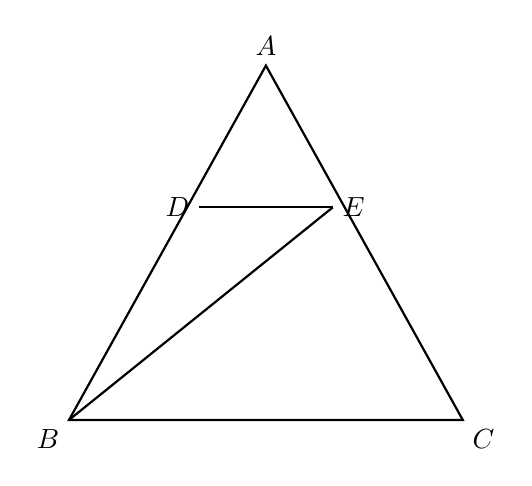
\begin{tikzpicture}
  \coordinate (A) at (2.5,4.5);
  \coordinate (B) at (0,0);
  \coordinate (C) at (5,0);
  \coordinate (D) at (1.65,2.7);
  \coordinate (E) at (3.35,2.7);

  \draw[thick] (A) -- (B) -- (C) -- cycle;
  \draw[thick] (D) -- (E);
  \draw[thick] (B) -- (E);

  \node[above] at (A) {$A$};
  \node[below left] at (B) {$B$};
  \node[below right] at (C) {$C$};
  \node[left] at (D) {$D$};
  \node[right] at (E) {$E$};
\end{tikzpicture}
\end{document}
